\subsection{Population Generator}
\begin{center}
    \textit{Terrain, Population markers} $\rightarrow$ \textbf{PopulationGenerator} $\rightarrow$ \textit{Population map} 
\end{center}
The population generator is responsible for creating an intensity map describing the population in the world.
Areas with higher intensity means there is a higher density of the population there.
Multiple generators in the sequence requires a population map in order to create more realistic buildings, thus the population map needs to reflect the landscape accordingly.
Because of that, the population map is responsible for the rough shape of the city.

In order to generate an intensity map, first it requires the terrain parameter, which is used to mask off certain areas in the landscape, such as oceans, rivers or mountains.
Then, the generator will use a few layers of simplex noise to create a representation of populations throughout the world.
Population markers are used to increase population density in a certain area, and these are applied after generating the initial population map.
This is useful for making sure the center of cities have a higher density, but it will still respect the original population map to some degree.

\begin{figure}[h]
  \centering
  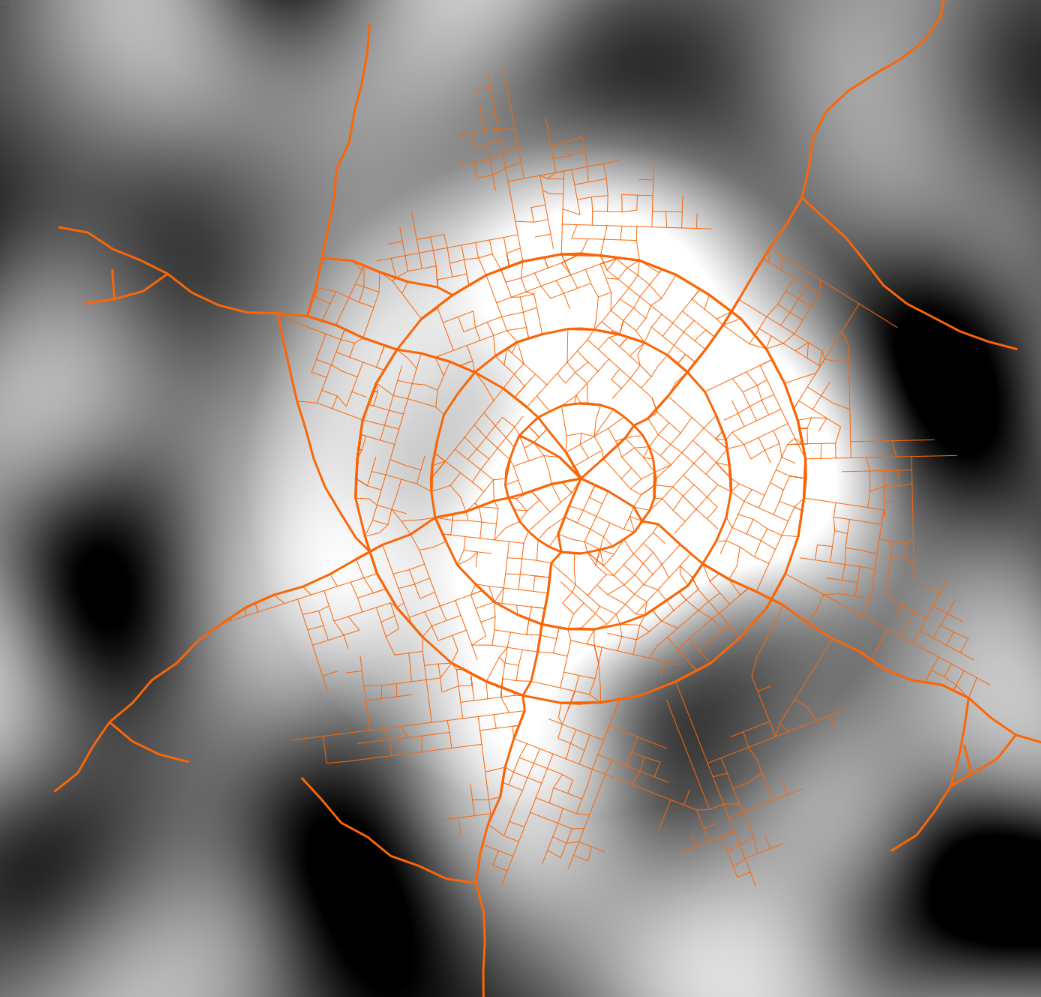
\includegraphics[width=0.6\textwidth]{figure/gen_population_map.png}
  \caption{An example of a population map with a Paris city generated within it}
  \label{fig:gen_population_map_example}
\end{figure}

In figure~\ref{fig:gen_population_map_example}, a population marker was placed in the center of the city, which means the population density is much higher there.
White areas have a higher population density, dark areas have a lower population density.
This figure also shows that main roads outside the cities will tend to shy away from lower density areas, but not always.
